\chapter{Application design}

\section{The real-world problem}
The Romanian national railway operator, CFR S.A. is tasked with the upkeep of 20 thousand kilometers of un-electrified and electrified railway spread out over 9 main lines \cite{CFROrdinMagistrale} \cite{WallstreetRoReorganizareSNCFR}, stretching all across Romania.

\begin{figure}[htbp]
    \centering
    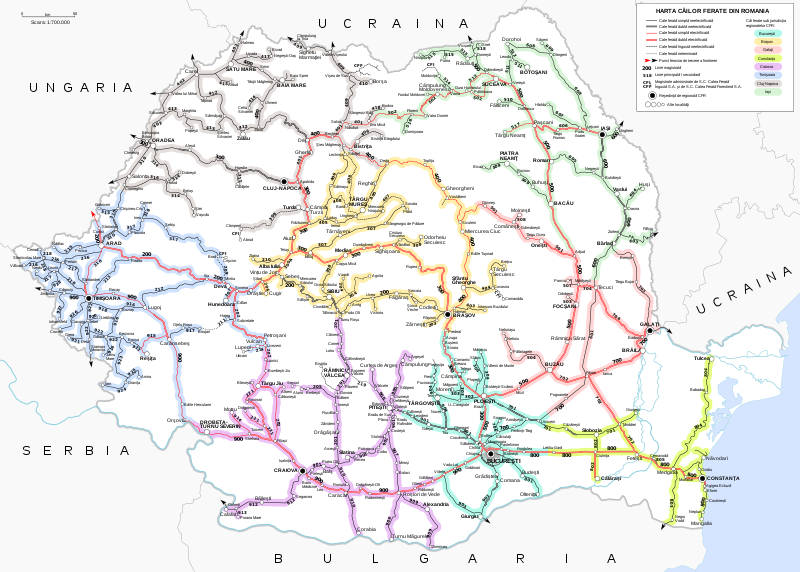
\includegraphics[width=0.8\textwidth]{./figures/ch3_romania-feroviara.png}
    \caption{Map of Romania's railway network. Map by Aero Avalon, shared under CC-BY 4.0 \cite{WikipediaRomaniaFeroviara}.}
    \label{FigRomaniaFeroviara}
\end{figure}

The passenger subsidiary, CFR Călători, is the biggest railway operator that makes use of these lines. However, rolling stock is outdated and most train cars lack modern features like driver-controlled doors. A notable absence though is that of live travel information offered inside the train to the passengers. An example of such an information display is given in Figure \ref{FigMAVInterior}.

\begin{figure}[htbp]
    \centering
    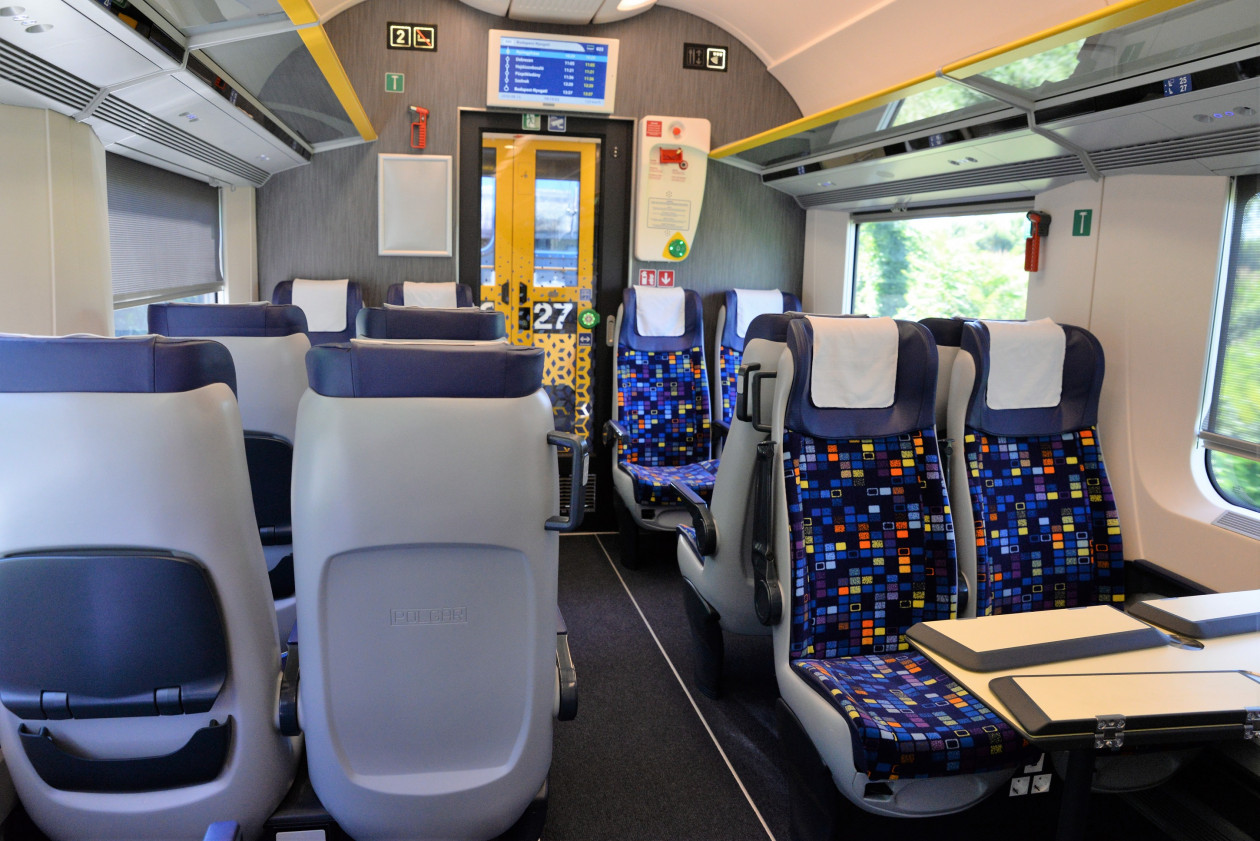
\includegraphics[width=0.8\textwidth]{./figures/ch1_mav-interior.png}
    \caption{Interior of a train owned by MÁV-Start, the Hungarian national passenger operator \cite{PestiHirlapMAVInterior}. The LCD display can be seen at the top, providing information about the next stations, times and delays. Stations and times can be pre-programmed into the train on departure, but delays require live integration with a central service.}
    \label{FigMAVInterior}
\end{figure}

Given that retrofitting all rolling stock with displays connected to the Internet is a challenging task, CFR Călători has attempted digitization in various other ways.

In 2016, the company launched IRIS, a web application that provided traffic information about the company's trains. It also offered information about delays \cite{StiriDeClujLansareCFRIris}. In 2018, IRIS got discontinued in favor of a newer platform, written in ASP.NET, which offers information about all railway operators in Romania.

In 2021, the company launched a mobile application with all the capabilities that the website has, making it more convenient than ever before to view traffic information \cite{MobilissimoCFRLansareMobil}.

These solutions, however, are insufficient in answering the question of "Where am I?" that a passenger might have. The most significant issue is that they all require Internet, the lack of which is an issue prevalent across Romanian trains \cite{CFRInternetIC}.

Moreover, CFR does not track the location of their trains using GPS transponders or any similar technology, but rather using personnel that are responsible with coordinating the trains passing through each station. This brings a number of issues:

\begin{itemize}
    \item \textbf{Data is not real-time.} A train passing through a station is only recorded when the station personnel manually records that train as passed, in the company's internal services.
    \item \textbf{Data might be missing.} Some personnel might not take the time to enter delay data for each passing train.
    \item \textbf{Some stations are not tracked.} Some train stations are big enough to be serviced by regional trains, but not big enough to warrant any personnel responsible with train movement.
    \item \textbf{Data might be false.} Station personnel can enter any delay data they want, having the possibility of hiding delays.
\end{itemize}

\section{Application requirements}
\label{sec:Requirements}

Given the set of real-world issues mentioned above, we can create a set of requirements for an application that tries to plug the information gap and provide a seamless travel experience for the passenger.

The basic idea of this thesis is to merge the mobile app experience and the website experience offered by CFR into a single solution, that will then be extended to offer live traffic information using phone capabilities such as the camera and location.

\begin{enumerate}
    \item Train trip information
          \begin{itemize}
              \item The app should allow the user to create a new trip. The user will be able to view live information about this trip.
              \item The app should be able to show details about the user's current position in their trip, using information obtained from user (train ticket), train database (itinerary of train) and phone sensors (GPS location).
              \item The live information should include: next stop, last stop, next stop arrival time (timetabled), train delay, next station of pass-through (if applicable).
              \item The live information may also include the destination arrival time (time\-tabled) + train delay.
              \item Information about the train ticket can be obtained using multiple methods: scanning the QR code of the ticket (state operator only), or manually inputting ticket data (train number, destination station).
              \item Access to non-live data should be provided via links to the Mersul Trenu\-rilor website (train itinerary, station stops).
              \item National train itinerary information will be saved to the user's device on application install. The information can be updated from the server. Attempts to automatically update this data will be done weekly.
          \end{itemize}
    \item User profile and authentication
          \begin{itemize}
              \item The app should be able to be used anonymously, without login. If so, persistent data must be saved locally to the device.
              \item The app must provide social login (login with Google, login with Apple) as the primary means of logging in.
              \item When creating a new account (logging in for the first time), if there is local data on the device, the app must offer the user the possibility of migrating it to the account. If logging into an existing account, local data must be deleted.
              \item The app must be able to show to the user a history of their trips.
              \item Logging in on another device will log out the already-logged-in device.
          \end{itemize}
    \item Connectivity
          \begin{itemize}
              \item The app must work without Internet, except for functionalities that directly require it.
              \item Account login will not work without Internet.
          \end{itemize}
          \item{Internationalization}
          \begin{itemize}
              \item The app must provide multi-language support (Romanian and English).
          \end{itemize}
\end{enumerate}

\section{Guiding principles}

To maximize user adoption and ease of use, the application should be centered about these core principles:

\begin{itemize}
    \item \textbf{Offline:} it will work at maximum capability while offline.
    \item \textbf{Easy to get into:} users should be able to get live tracking as soon as they click a link, and should not have to install apps.
    \item \textbf{Live information:} the screen will update as soon as the app gets new traffic or position information.
    \item \textbf{Information at a glance:} all information needed to answer the questions of "Where am I?", "How long until next stop?", "How long until my stop?" is always displayed on-screen.
    \item \textbf{Minimal configuration:} integrate with existing CFR services and ticketing systems as seamlessly as possible.
    \item \textbf{Avoid "yet another account and password":} allow the user to save their preferences locally, or use social login to sync them. Do not ask the user to remember another password!
\end{itemize}

\section{Use case diagram}

We can design an use case diagram showing the main functionalities of the application and how we intend them to interoperate and operate with the various actors, in Figure \ref{FigUseCase}.

\begin{figure}[htbp]
    \centering
    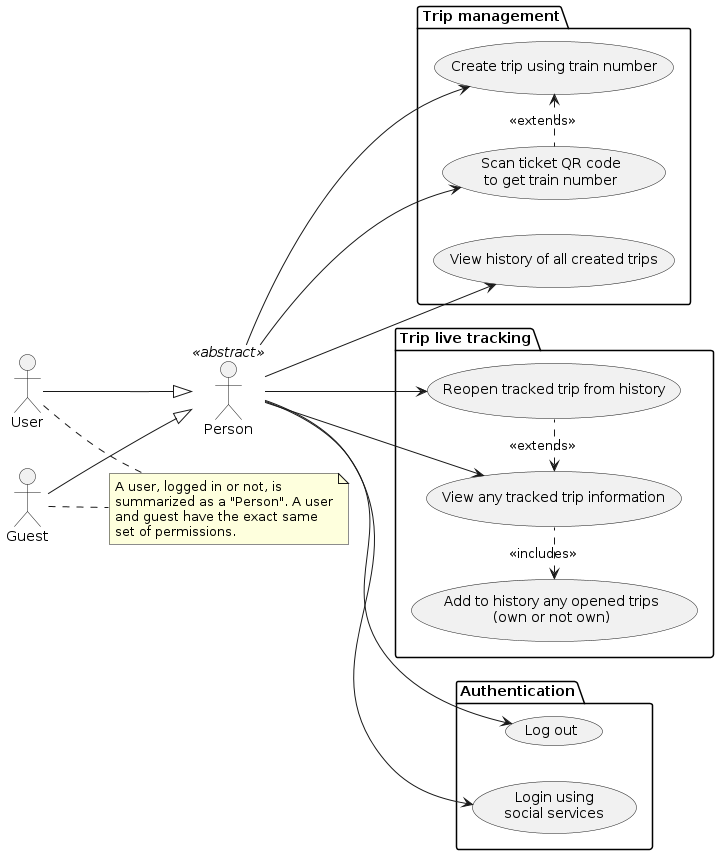
\includegraphics[width=0.9\textwidth]{./figures/ch3_use-case.png}
    \caption{Use case diagram for our CFR Companion application.}
    \label{FigUseCase}
\end{figure}

As you can see, even though user accounts are employed, there is little operational difference between users that are logged in, and those who are not. The permission set is the same, what is different is where the user data (trip history) is saved.

\section{Architecture considerations}
As a summary of Chapter 2, we can provide a short comparison between possible architectures:

\begin{enumerate}
    \item Native application
          \begin{itemize}
              \item Requires distribution on multiple marketplaces (Google Play Store, Apple App Store).
              \item Requires multiple builds (for each supported platform: iOS, Android).
              \item Installation necessary.
              \item Internet not required for base functionality.
          \end{itemize}
    \item Web application
          \begin{itemize}
              \item Distribution is straightforward (accessing a link is sufficient).
              \item No installation necessary.
              \item Cross-platform by default.
              \item Internet required for base functionality.
          \end{itemize}
    \item Progressive Web Application
          \begin{itemize}
              \item Distribution is straightforward (accessing a link is sufficient).
              \item No installation necessary, although possible.
              \item Internet not required for base functionality (even if not installed).
          \end{itemize}
\end{enumerate}

Remarks relative to our product requirements (section \ref{sec:Requirements}):
\begin{enumerate}
    \item Our train companion app intends to be easy to use and access. Asking users to download and install a native application goes against this intention.
    \item Our train companion app must work without Internet. Asking users to access a website every time they want to use our application goes against this requirement.
\end{enumerate}

The choice of a Progressive Web Application architecture is therefore justified, since this resolves a series of drawbacks of both other possible architectures.

The employment of a backend is also needed, to provide a way of downloading up-to-date GTFS data, and provide support for user accounts (which are not required, moreover are impossible, to work offline).

\section{Underlying infrastructure}
\label{sec:Infrastructure}

Given our choice of PWA and the requirement of offline functionality, the infrastructure of our application will take a shape similar to Figure \ref{FigGenericComponentDiagram}.

This layout does not conform to the classic Single Page Application (SPA) architecture, where the frontend is but a shell over a backend and the backend is but a shell in front of a database. We have to make use of a local database, which will serve as the place where we store all local data, such as train itineraries and user preferences.

\begin{figure}[htbp]
    \centering
    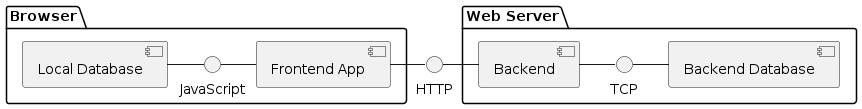
\includegraphics[width=\textwidth]{./figures/ch3_component-diagram.png}
    \caption{Generic component diagram for our application, with no specific software in mind.}
    \label{FigGenericComponentDiagram}
\end{figure}

By analyzing software options for our various infrastructure requirements, we come to the following conclusions:

\begin{enumerate}
    \item \textbf{Local database:} modern browsers and Web standards offer various tools for client-side persistent storage. The most widely known, cookies, are not suitable for this application, since the scale of data we need to store (train itinera\-ries) easily blows over storage quotas of cookies. We must also keep in mind that cookies are not necessarily suitable for client-side access, and are mostly useful as identification tokens for backend systems. We turn then to local storage, which provides a global key-value store for our page. This would work, but we have an even better, more RDBMS-like solution: \textbf{IndexedDB}! This standard provides us tools to interact with data stores called \textit{databases}, create \textit{tables} and define \textit{indexes} on them. This also makes for a convenient place to store other data, such as user preferences.
    \item \textbf{Frontend application:} this discussion is broad, and while many frameworks have their advantages and disadvantages, I think it is ultimately resumed to developer preference. I chose to develop the frontend using \textbf{React}, and have \textbf{Vite} act as a bundler. Vite offers plugins to easily convert React SPAs into proper installable PWAs, so it was an easy decision from this standpoint.
    \item \textbf{Backend application:} this discussion is even broader than the frontend one. I chose to use \textbf{TypeScript} as the language, and \textbf{NestJS} as a framework to build my API in. NestJS provides an excellent developer experience, and having both frontend and backend languages be similar provides a lot of benefit.
    \item \textbf{Backend database:} there are a lot of factors to consider for a database, such as maximum traffic requirements, data access speed requirements, data write speed requirements, schema integrity requirements. However, one development requirement for this application resides in \textit{cost}, which was the ultimate deciding factor for the backend database, since other concerns are not as stringent. For this reason, I have chosen \textbf{MongoDB} as a backend database, since their parent company provides an excellent database-as-a-service in the form of \textbf{MongoDB Atlas}, which has an excellent free tier. The serverless tier might also come in handy, for scalability concerns.
\end{enumerate}

\section{Entities}
\label{sec:Entities}
By parsing the requirements (section \ref{sec:Requirements}), we can identify a series of entities that the user must interact with. A breakdown of identified entities is provided in Figure \ref{FigDbDiagram}, which takes into account our two different database locations, as defined in the infrastructure section (\ref{sec:Infrastructure}).

\begin{figure}[htbp]
    \centering
    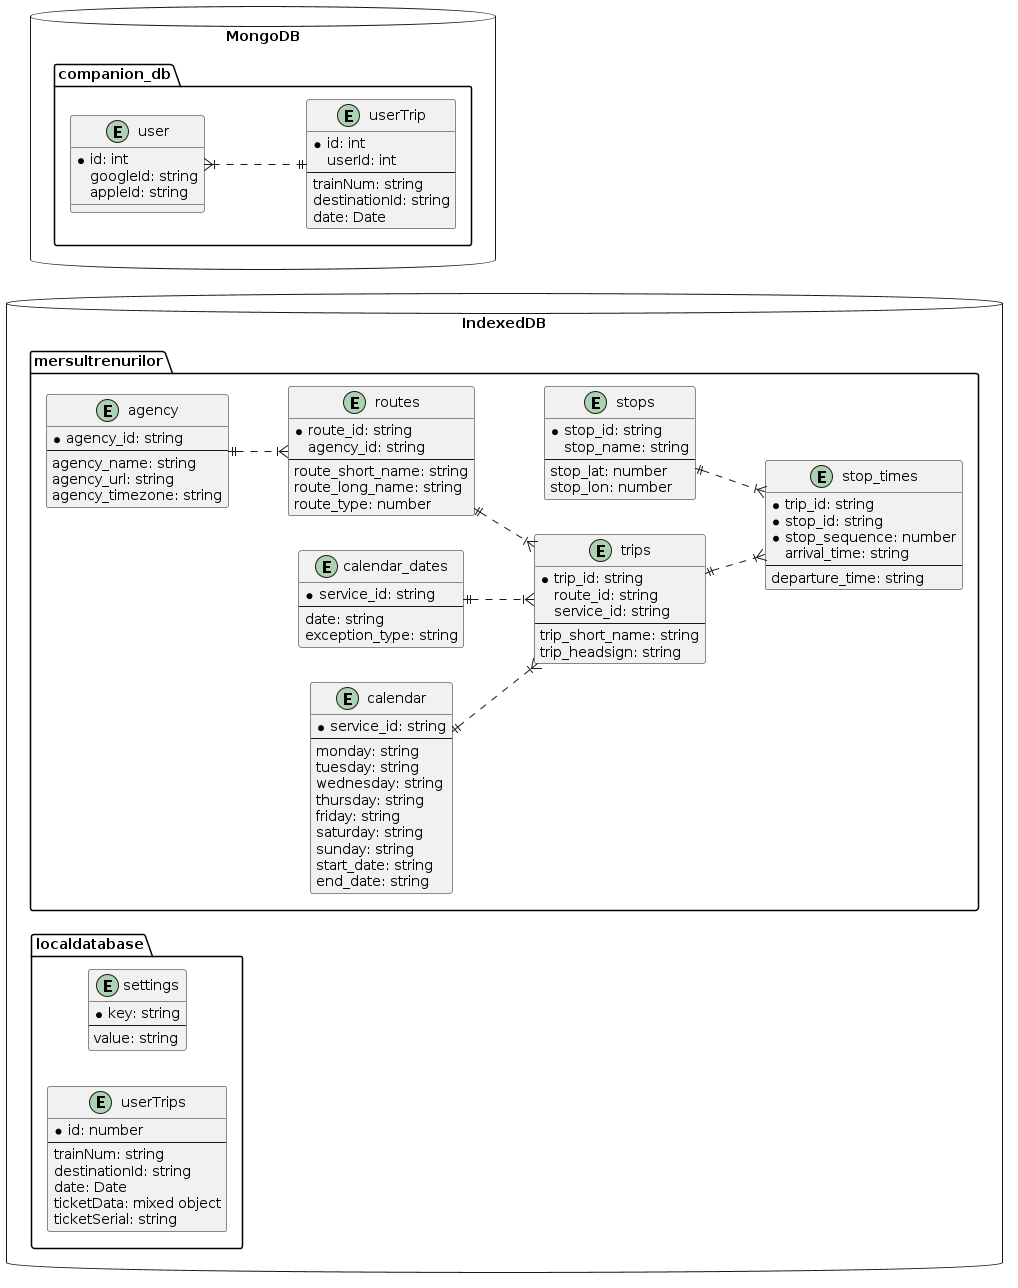
\includegraphics[width=1\textwidth]{./figures/ch3_db-diagram.png}
    \caption{Database diagram of both databases.}
    \label{FigDbDiagram}
\end{figure}

We recognize that CFR travel information must be stored, and for this, we must choose a suitable format. To this end, we can make use of the General Transit Feed Specification (GTFS) standard. In particular, we look at the GTFS Schedule variant, which provides static (schedule) information, without live data, and we can obtain the entities that our application needs from there.

From the GTFS Schedule reference, we make use of a subset of entities, enumerated in Table \ref{TableGTFS}. Notably, we omit entities related to fares, station layouts, translations, headways, since such information is not provided in the official CFR timetables.

An important note needs to be made regarding the GTFS format, in that we will not make use of text files in the way that the specification suggests. We will keep the schema of the text files, but instead of storing them as CSV files, we parse them and upload each item in its corresponding table in the IndexedDB \verb|mersultrenurilor| database.

\begin{table}[htbp]
    \centering
    \begin{tabular}{|m{0.25\textwidth}|m{.65\textwidth}|}
        \hline
        GTFS filename       & Description                                                                                                          \\
        \hline
        agency.txt          & The railway operators in Romania, which includes the national operator CFR along with a couple of private operators. \\
        \hline
        stops.txt           & All stations.                                                                                                        \\
        \hline
        routes.txt          & Transit routes. A route is a group of trips that are displayed to passengers as a single service.                    \\
        \hline
        trips.txt           & Trips for each route. A trip is a sequence of two or more stops that occur during a specific time period.            \\
        \hline
        stop\_times.txt     & Times that a train arrives at and departs from stops for each trip.                                                  \\
        \hline
        calendar.txt        & Service dates specified using a weekly schedule with start and end dates.                                            \\
        \hline
        calendar\_dates.txt & Exceptions for the services defined in the calendar.txt.                                                             \\
        \hline
    \end{tabular}
    \caption{GTFS Schedule data that we are going to make use of.}
    \label{TableGTFS}
\end{table}

\section{Location of GTFS travel data}

The question of where to store the GTFS travel information is one that easily finds its answer in the frontend database, for the simple reason that the requirements (Section \ref{sec:Requirements}) mandate that this travel information be available offline.

Having the GTFS travel data available offline brings a number of advantages, such as:
\begin{enumerate}
    \item Accessing the data is blazing fast and not subject to (extremely variable) network latency.
    \item A step of abstraction, in the form of an Internet API, is not needed, reducing complexity.
\end{enumerate}

Conversely, storing the data offline is disadvantageous because:
\begin{enumerate}
    \setcounter{enumi}{2}
    \item There might not be suitable browser functionality to store this data with.
    \item The dataset might be too large to store.
    \item The dataset might take too long to download.
\end{enumerate}

However, these disadvantages (and potential disadvantages) can be mitigated using the following methods (and arguments):
\begin{enumerate}
    \setcounter{enumi}{5}
    \item \textbf{(For 3)} A suitable place to store large amounts of data \textit{does} exist, in the form of IndexedDB \cite{IndexedDBIntro}.
    \item \textbf{(For 4)} The IndexedDB quotas easily fit around the size of our GTFS dataset \cite{IndexedDBLimits}.
    \item \textbf{(For 5)} Mitigating long download times is not wholly possible, but we can make the user aware of when travel data is downloading, and implement caching strategies both client-side and server-side, to alleviate this issue.
\end{enumerate}

We also need to store trip history information in the user's browser. Although this can easily be accomplished using other storage methods such as Local Storage, we already made use of IndexedDB, therefore we can just create a separate database to the GTFS data and store our trip history there.

As part of our caching strategy for the disadvantage with number 5 mentioned above, we also need to store when the last travel data was downloaded.

\section{Sourcing of the GTFS travel data}

Although Romanian train operators publish their travel data annually \cite{DataGovRoDespre} \cite{DataGovRoLicense}, the data comes in a monolithic non-standard XML file, that is directly unusable for our application.

We use the GTFS format for our application because it is structured on "tables", is widely supported and is very easily indexable. Therefore, we must find a way to convert this XML data to GTFS.

Thankfully, such a converter already exists, in the form of Vasile Cotovanu's GTFS exporter \cite{VasileRubyExporter} written in Ruby and published on his GitHub account that has the wonderful handle of \verb|vasile|.

Running the exporter produces a list of text files as detailed in Table \ref{TableGTFS}. Although the data is in a familiar tabular format, it is not easily parsable and indexable in this CSV form.
